\documentclass[11pt]{article}
\usepackage[T1]{fontenc}
\usepackage{lmodern}
\usepackage{amsmath,amssymb,amsthm,mathtools}
\usepackage[letterpaper,margin=1in]{geometry}
\usepackage{microtype}
\usepackage{enumitem}
\usepackage{booktabs}
\usepackage{graphicx}
\usepackage{tikz}
\usetikzlibrary{arrows.meta,calc,positioning}
\usepackage{xcolor}
\definecolor{linkblue}{HTML}{23527C}
\definecolor{parentblue}{HTML}{28698D}
\definecolor{childorange}{HTML}{B76223}
\usepackage[colorlinks=true,linkcolor=linkblue,citecolor=linkblue,urlcolor=linkblue]{hyperref}
\usepackage[capitalise,noabbrev]{cleveref}
\hypersetup{pdftitle={Thompson's group F is nonamenable}}

\newcommand{\R}{\mathbb R}
\newcommand{\N}{\mathbb N}
\newcommand{\Z}{\mathbb Z}
\newcommand{\norm}[1]{\lVert #1\rVert}
\newcommand{\ip}[2]{\langle #1,#2\rangle}
\newcommand{\id}{\mathrm{id}}
\DeclareMathOperator{\Lip}{Lip}
\DeclareMathOperator{\dist}{dist}
\DeclareMathOperator{\sinc}{sinc}
\newtheorem{theorem}{Theorem}[section]
\newtheorem{lemma}[theorem]{Lemma}
\newtheorem{proposition}[theorem]{Proposition}
\newtheorem{corollary}[theorem]{Corollary}
\theoremstyle{definition}
\newtheorem{definition}[theorem]{Definition}
\newtheorem{remark}[theorem]{Remark}
\numberwithin{equation}{section}
\setlist[itemize]{topsep=4pt,itemsep=2pt,parsep=0pt}
\setlist[enumerate]{topsep=4pt,itemsep=2pt,parsep=0pt}
\setlength{\emergencystretch}{2em}

\newcommand{\unverified}[1]{\par\smallskip\noindent\fbox{\parbox{0.95\linewidth}{\textbf{Unverified step.} #1}}\par\smallskip}
\newcommand{\step}[1]{\par\smallskip\noindent\textbf{Step #1.}\enspace}
\newcommand{\EA}{\mathbb E_A}

\title{Thompson's group \(F\) is nonamenable}
\author{Rewritten for readability from the OpenAI manuscript of the same title}
\date{September 23, 2026}

\begin{document}
\maketitle
\begin{abstract}
We prove that Thompson's group \(F\) is nonamenable. This confirms
Geoghegan's conjecture and resolves the amenability problem for \(F\).
\end{abstract}

\section{The result and the shape of the proof}
\label{sec:introduction}

\subsection{Statement}

\emph{Thompson's group} \(F\) consists of the increasing piecewise linear
homeomorphisms of \([0,1]\) with finitely many linear pieces, breakpoints at
dyadic rationals (numbers \(k/2^n\)), and slopes in \(2^{\Z}\). The group
operation is composition, written \(hg=h\circ g\) (apply \(g\) first), and \(F\)
is regarded as a discrete group.

A discrete group \(\Gamma\) is \emph{amenable} if its bounded real-valued
functions admit a positive normalized left-invariant mean: a linear
functional \(M:\ell^\infty(\Gamma;\R)\to\R\) with \(M(1)=1\),
\(M(\varphi)\ge0\) whenever \(\varphi\ge0\), and
\(M(g\mapsto\varphi(hg))=M(\varphi)\) for every \(h\in\Gamma\).
(The source writes \(G\) for a general group; we write \(\Gamma\) because
\(G\) denotes a map in the appendix.)
This viewpoint belongs to the classical theory of von Neumann and Day
\cite{vonNeumann1929,Day1957}.

\begin{theorem}\label{thm:main}
Thompson's group \(F\) is not amenable.
\end{theorem}

This is Geoghegan's 1979 conjecture, as recorded in
\cite[p.~227]{CannonFloydParry1996}.

\paragraph{The only fact about amenability that is used.}
We use the forward implication of the F\o lner criterion
\cite{Folner1955}: \emph{if \(\Gamma\) is amenable, then for every finite
\(S\subset \Gamma\) and every \(\varepsilon>0\) there is a nonempty finite
\(A\subset \Gamma\) such that}
\begin{equation}\label{eq:folner}
  \frac{|hA\mathbin{\triangle}A|}{|A|}<\varepsilon
  \qquad(h\in S).
\end{equation}
Here \(hA=\{hg:g\in A\}\) and \(\triangle\) is the symmetric difference.
The modern left-translation formulation in
\cite[Theorem~1.2]{Moore2013} bounds the sum over \(h\in S\) of these
ratios. Applying it with a smaller tolerance (say \(\varepsilon/2\)) gives
each individual strict bound in \eqref{eq:folner}.
So, to prove \cref{thm:main}, it suffices to find one finite
\(S\subset F\) and one constant \(c_0>0\) such that
\(\max_{h\in S}|hA\triangle A|/|A|\ge c_0\) for \emph{every} nonempty
finite \(A\subset F\). This is \cref{avg:boundary}.

\subsection{The one analytic input}

\begin{lemma}[Benyamini--Sternfeld]\label{lem:displacement}
There are a real Hilbert space \(H\), a Lipschitz map \(f:B\to B\) on its
closed unit ball \(B\), and a constant \(\delta>0\) such that
\[
  \norm{f(x)-x}\ge\delta\qquad(x\in B).
\]
\end{lemma}

Benyamini and Sternfeld prove this for every infinite-dimensional
normed space \cite[Theorem, part~(3), p.~439]{BenyaminiSternfeld1983}.
\Cref{app:auxiliary} gives a self-contained construction on
\(L^2([0,1];\R^2)\) with \(\delta=1/2\).
\emph{Sanity check.} No such \(f\) exists when \(\dim H<\infty\), since
Brouwer's theorem gives a fixed point. This is why the proof below needs
Hilbert-valued, not scalar, colours.
\Cref{lem:displacement} is used exactly once, in
\eqref{avg:displacement}.

\subsection{Proof at a glance}\label{sec:glance}

\paragraph{Key idea.}
Let \(f,L,\delta\) be as in \cref{lem:displacement} (\(L\) a Lipschitz
constant of \(f\)) and let \(D\) be a large integer.
To each \(g\in F\) we attach finitely many vectors \(X_I(g)\in B\),
indexed by intervals \(I\). They satisfy an \emph{exact nonlinear recursion}
through \(f\). Their pairwise inner products are also \emph{exactly
transported} by suitable elements of \(F\).
If a finite set \(A\subset F\) were almost invariant under those elements,
all these inner products would have nearly the same average over \(A\).
A two-line Hilbert-space computation would then turn the recursion into an
approximate fixed point of \(f\), which \cref{lem:displacement} forbids.

\paragraph{Objects (defined precisely in \cref{sec:dyadic,sec:coloring}).}
\begin{itemize}
\item A \emph{basic partition} is a finite partition of \([0,1]\) into
dyadic intervals \([k2^{-r},(k+1)2^{-r}]\). For \(g\in F\) and large \(n\),
the image \(gT^{(n)}\) of the uniform level-\(n\) partition is basic.
\item Fix \(D\) \emph{parent} intervals \(I_1<\dots<I_D\) with gaps between
them, inside \((0,1)\). Inside each parent \(I_i\) put the affine copy of the
same family; this gives \(D^2\) \emph{descendants} \(I_i\cdot I_j\).
\item A \emph{colouring} \(p\) assigns to every basic partition \(T\) a
vector \(p(T)\in B\) by recursion on the number of cells. If \(T\) is fine
enough, \(p(T)=f(\text{mean of the colours of the }D\text{ pieces of }T
\text{ in }I_1,\dots,I_D\text{, each rescaled to }[0,1])\). Otherwise
\(p(T)=0\).
\item \(X_I(g)\) is the colour of the piece of \(gT^{(n)}\) in \(I\),
rescaled to \([0,1]\).
\end{itemize}

\paragraph{Steps and dependencies.}
\begin{enumerate}[label=(\arabic*)]
\item \emph{Recursion identity (exact).}
\(X_{I_i}(g)=f(z_i(g))\), where \(z_i(g)=\frac1D\sum_j X_{I_i\cdot I_j}(g)\).
Uses \cref{dyad:restr}(c) and the definition of \(p\) (\cref{color:wd}).
\item \emph{Transport (exact).}
If \(h\in F\) maps \(I\) affinely onto \(I'\), then \(X_I(g)=X_{I'}(hg)\)
(\cref{dyad:cov}). For every pair \(I<J\) of our intervals with a gap
between them, \(F\) contains an element \(h_{I,J}\) mapping \(I\to I_1\) and
\(J\to I_2\) affinely (\cref{dyad:transport}). The finite set \(S\) of these
elements is fixed before \(A\).
\item \emph{Equal correlations.}
Let \(\eta=\max_{h\in S}|hA\triangle A|/|A|\) and
\(\alpha=\EA\ip{X_{I_1}}{X_{I_2}}\) (average over \(A\)).
Then \(|\EA\ip{X_I}{X_J}-\alpha|\le\eta\) for every such pair.
Uses (2), the list of separated pairs (\cref{color:pairs}) and the counting
\cref{avg:translation}.
\item \emph{Variance estimate.}
With \(m=\frac1D\sum_kX_{I_k}\), expanding
\(\norm{z_i-m}^2\) and using (3) on all but a fraction \(1/D\) of the
inner products gives
\(\EA\norm{z_i-m}^2\le 4/D+4(1-1/D)\eta\); the unknown \(\alpha\)
cancels.
\item \emph{Contradiction with displacement.}
By (1), \(m=\frac1D\sum_i f(z_i)\), so
\(\delta^2\le\norm{m-f(m)}^2\le\frac{L^2}{D}\sum_i\norm{z_i-m}^2\).
Averaging over \(A\) and inserting (4) gives
\(\delta^2\le L^2\bigl(4/D+4(1-1/D)\eta\bigr)\). For \(D>4L^2/\delta^2\)
this is a positive lower bound on \(\eta\) independent of \(A\)
(\cref{avg:boundary}), contradicting \eqref{eq:folner}.
\end{enumerate}
The level \(n\) is chosen after \(A\), so that all partitions involved are
fine enough (\cref{dyad:eventual}). This is harmless because \(S\) and the
final constant do not depend on \(n\).
\Cref{sec:consequences} records two consequences that rely on separate
companion theorems. \Cref{app:auxiliary} proves \cref{lem:displacement}.

\subsection{Context and prior work}
This subsection is background and is not used in the proof.

Thompson introduced \(F\) in 1965; an early published construction appears
in McKenzie and Thompson \cite{McKenzieThompson1973}, with the identification
explained by Cannon, Floyd, and Parry \cite[pp.~215--216]{CannonFloydParry1996}.
Two classical structural facts help explain the difficulty of the
amenability problem. Brin and Squier show that \(F\) contains no
nonabelian free subgroup \cite[Theorem~3.1]{BrinSquier1985}, so the familiar
free-subgroup obstruction does not apply. Yet \(F\) is not elementary
amenable \cite[Theorem~4.10]{CannonFloydParry1996}: it lies outside the class
generated by finite and abelian groups under subgroups, quotients,
extensions, and directed unions. Neither fact decides ordinary
amenability. Brown and Geoghegan construct a classifying space with finitely
many cells in each dimension \cite{BrownGeoghegan1984}.

Moore proves tower lower bounds on the sizes of possible
F\o lner sets \cite[Theorem~1.1]{MooreFolner2013} and characterizes
amenability of \(F\) by a scalar convex Ramsey property for finite rooted
ordered binary trees \cite[Theorem~3.1]{Moore2013}. Guba improves densities
of finite Cayley subgraphs \cite{Guba2025Density} and derives restrictions
on right-invariant means from a partition into seven diagram-defined
classes \cite{Guba2026}. Haagerup and Olesen prove that simplicity of the
reduced group \(C^*\)-algebra of Thompson's group \(T\) would imply
nonamenability of \(F\) \cite[Theorem~5.5]{HaagerupOlesen2017}.
The proof below uses finite dyadic partitions and scalar correlations of
Hilbert-valued colours.

There have also been claims of a complete resolution in both directions.
Akhmedov's 2021 version claims nonamenability through a height-function
criterion \cite{Akhmedov2021}. Shavgulidze claimed amenability
\cite{Shavgulidze2009}; Moore identified errors in that approach
\cite{Moore2011Critique}. Moore separately withdrew an amenability claim
after Akhmedov identified an error in Lemma~4.13 of that manuscript
\cite{Moore2012Withdrawn}. That withdrawal concerns a different work from
his published Ramsey characterization cited above.

\section{Dyadic partitions and affine transport}\label{sec:dyadic}

We use the standard dyadic-partition model of \(F\); see
\cite[Section~2, Lemma~2.2]{CannonFloydParry1996}. Everything needed is
proved here.

\subsection{Definitions}

\begin{itemize}
\item A \emph{basic (dyadic) interval} is an interval
\([k2^{-r},(k+1)2^{-r}]\subseteq[0,1]\) with \(r\in\N\cup\{0\}\) and
\(0\le k<2^r\).
\item A \emph{basic partition} is a finite family of basic intervals
(\emph{cells}) with union \([0,1]\) and pairwise disjoint interiors; cells
may share endpoints. Its \emph{mesh} is the greatest length of a cell.
\(T^{(n)}\) denotes the uniform partition into the \(2^n\) cells of length
\(2^{-n}\).
\item A partition \(T\) \emph{respects} an interval \(I\) if \(I\) is a
union of cells of \(T\).
\item For a basic interval \(I\), \(s_I:[0,1]\to I\) is the increasing
affine bijection, and \(I\cdot J=s_I(J)\) for a basic interval \(J\).
\item If \(T\) respects \(I\), its \emph{normalized restriction} is
\(T_I=\{s_I^{-1}(C):C\in T,\ C\subseteq I\}\).
\item \(I<J\) means \(\max I<\min J\); this requires a positive gap. We
then call \(I,J\) \emph{strictly separated}. An interval is \emph{internal}
if both endpoints lie in \((0,1)\).
\item \(h\in F\) \emph{carries \(I\) affinely onto \(I'\)} if \(h|_I\) is
affine and \(h(I)=I'\). Since \(h\) is increasing, \(h\circ s_I\) is then an
increasing affine bijection \([0,1]\to I'\), so
\begin{equation}\label{dyad:chart}
  h\circ s_I=s_{I'}.
\end{equation}
\item For \(g\in F\), \(gT^{(n)}=\{g(C):C\in T^{(n)}\}\).
\end{itemize}

\emph{Example.} For \(I=[\tfrac14,\tfrac12]\) and \(J=[\tfrac12,1]\) we get
\(I\cdot J=[\tfrac38,\tfrac12]\). The partition \(T^{(3)}\) respects \(I\),
and \((T^{(3)})_I=T^{(1)}\).

\subsection{Normalized restrictions}

The next lemma is used to show that the colouring is well defined
(\cref{color:wd}) and to prove the recursion identity
\eqref{avg:recursive-identity}.

\begin{lemma}\label{dyad:restr}
Let \(I,J\) be basic intervals and \(T\) a basic partition.
\begin{enumerate}[label=(\alph*)]
\item \(I\cdot J\) is a basic interval contained in \(I\), and
\(s_{I\cdot J}=s_I\circ s_J\).
\item If \(T\) respects \(I\), then \(T_I\) is a basic partition, with
exactly as many cells as \(T\) has cells contained in \(I\).
\item If \(T\) respects both \(I\) and \(I\cdot J\), then \(T_I\) respects
\(J\) and
\begin{equation}\label{dyad:restriction}
  (T_I)_J=T_{I\cdot J}.
\end{equation}
\end{enumerate}
\end{lemma}

\begin{proof}
Write \(I=[k2^{-r},(k+1)2^{-r}]\), so \(s_I(x)=2^{-r}(x+k)\) and
\(s_I^{-1}(y)=2^ry-k\).

(a) If \(J=[k'2^{-r'},(k'+1)2^{-r'}]\), then
\(s_I(J)=[(k2^{r'}+k')2^{-(r+r')},(k2^{r'}+k'+1)2^{-(r+r')}]\), a basic
interval inside \(s_I([0,1])=I\). The map \(s_I\circ s_J\) is increasing,
affine, and maps \([0,1]\) onto \(s_I(J)=I\cdot J\); such a map is unique,
so it equals \(s_{I\cdot J}\).

(b) Let \(C=[j2^{-\ell},(j+1)2^{-\ell}]\) be a cell of \(T\) with
\(C\subseteq I\). Then \(\ell\ge r\), and
\(s_I^{-1}(C)=[(j-k2^{\ell-r})2^{-(\ell-r)},(j-k2^{\ell-r}+1)2^{-(\ell-r)}]\).
Its left endpoint is an integer multiple of its length \(2^{-(\ell-r)}\), and
it lies in \(s_I^{-1}(I)=[0,1]\), so it is basic. Because \(I\) is the union
of the cells \(C\subseteq I\), their images cover \([0,1]\). Their interiors
are disjoint because \(s_I^{-1}\) is injective. Injectivity also gives the
count of cells.

(c) By (a), \(I\cdot J\subseteq I\), so the cells of \(T\) contained in
\(I\cdot J\) are among those contained in \(I\). Since \(T\) respects
\(I\cdot J\), we get
\(J=s_I^{-1}(I\cdot J)=\bigcup\{s_I^{-1}(C):C\in T,\ C\subseteq I\cdot J\}\),
a union of cells of \(T_I\). So \(T_I\) respects \(J\). A cell
\(s_I^{-1}(C)\) of \(T_I\) lies in \(J\) exactly when \(C\subseteq
s_I(J)=I\cdot J\). Hence, using (a),
\[
 (T_I)_J=\{s_J^{-1}s_I^{-1}(C):C\in T,\ C\subseteq I\cdot J\}
        =\{s_{I\cdot J}^{-1}(C):C\in T,\ C\subseteq I\cdot J\}
        =T_{I\cdot J}.\qedhere
\]
\end{proof}

\subsection{Images of fine uniform partitions}

The next lemma is used once, in the proof of \cref{avg:boundary}, to choose
the level \(n\).

\begin{lemma}\label{dyad:eventual}
For each \(g\in F\), the partitions \(gT^{(n)}\) are basic for all
sufficiently large \(n\), and their meshes tend to zero. In particular,
given a finite set \(E\subset F\) and a finite family \(\mathcal J\) of
basic intervals, there is an \(n_0\) such that \(gT^{(n)}\) is basic and
respects every member of \(\mathcal J\) whenever \(g\in E\) and
\(n\ge n_0\).
\end{lemma}

\begin{proof}
\step{1 (form of the pieces)}
Let \(0=x_0<x_1<\dots<x_N=1\) be dyadic points containing all breakpoints
of \(g\), and let \(2^{q_i}\) be the slope on \([x_{i-1},x_i]\). Since
\(g(0)=0\), we have \(g(x_i)=\sum_{j\le i}2^{q_j}(x_j-x_{j-1})\), a dyadic
rational. Hence on the \(i\)-th piece \(g(x)=2^{q_i}x+b_i\) with
\(b_i=g(x_{i-1})-2^{q_i}x_{i-1}\) dyadic.

\step{2 (\(gT^{(n)}\) is basic for large \(n\))}
Choose \(n\) so large that (i) every \(x_i\) is a multiple of \(2^{-n}\),
(ii) \(n\ge q_i\) for all \(i\), and (iii) every \(b_i\) is an integer
multiple of \(2^{q_i-n}\). Each condition, once true, stays true for
larger \(n\), and there are finitely many pieces. By (i), every cell
\([k2^{-n},(k+1)2^{-n}]\) lies in one piece, say the \(i\)-th. Its image is
\([k''2^{q_i-n},(k''+1)2^{q_i-n}]\) with \(k''=k+b_i2^{n-q_i}\), an integer
by (iii). The length \(2^{-(n-q_i)}\) is at most \(1\) by (ii), and the
image lies in \([0,1]\), so it is a basic interval. As \(g\) is a
homeomorphism of \([0,1]\), the images form a partition.

\step{3 (mesh)}
The mesh of \(gT^{(n)}\) is \(2^{\max_iq_i-n}\to0\).

\step{4 (basic intervals with intersecting interiors are nested)}
Let \(I',I''\) be basic of lengths \(2^{-r'}\ge2^{-r''}\). Every endpoint of
\(T^{(r')}\) is a multiple of \(2^{-r''}\), so none lies in the interior of
\(I''\). Thus \(I''\) lies in a single cell of \(T^{(r')}\). If the
interiors of \(I'\) and \(I''\) meet, that cell must be \(I'\), so
\(I''\subseteq I'\).

\step{5 (small mesh implies respect)}
Let \(T\) be a basic partition of mesh smaller than the length of a basic
interval \(I\). Take \(x\) in the interior of \(I\) and a cell \(C\ni x\).
Since \(C\) is a nondegenerate interval, its interior meets that of \(I\).
By Step~4 the two are nested, and \(C\) is shorter, so \(C\subseteq I\).
Hence the interior of \(I\) lies in the union of the cells contained in
\(I\). That union is closed and contained in \(I\), so it equals \(I\).

\step{6 (conclusion)}
For each \(g\in E\), Steps 2, 3 and 5 give a threshold beyond which
\(gT^{(n)}\) is basic with mesh below the shortest member of
\(\mathcal J\), hence respects every member. Take \(n_0\) to be the largest
of these finitely many thresholds.
\end{proof}

\subsection{Transport of pairs and exact covariance}

The next lemma supplies the finite set \(S\) of \cref{sec:boundary}.

\begin{lemma}\label{dyad:transport}
If \(I<J\) and \(I'<J'\) are pairs of internal basic intervals, there is
an \(h\in F\) carrying \(I\) affinely onto \(I'\) and \(J\) affinely onto
\(J'\).
\end{lemma}

\begin{proof}
\step{1 (gaps)}
The source pair leaves three gaps \([0,\min I]\), \([\max I,\min J]\),
\([\max J,1]\). Each has positive length because \(I,J\) are internal and
\(I<J\), and each has dyadic endpoints. The same holds for the target pair.

\step{2 (partition the gaps)}
Choose \(N\) with all endpoints of the six gaps multiples of \(2^{-N}\);
then each gap is a union of cells of \(T^{(N)}\), which are basic.

\step{3 (equalize)}
For each of the three positions, if the source gap has fewer cells than the
corresponding target gap (or conversely), bisect one cell on the side with
fewer cells. The two halves of a basic interval are basic and the number of
cells increases by one. Repeat until the numbers agree.

\step{4 (define \(h\))}
Now the list (cells of gap 1, \(I\), cells of gap 2, \(J\), cells of gap 3)
and the corresponding target list are basic partitions of \([0,1]\) with the
same number of cells, with \(I,J\) and \(I',J'\) in matching positions.
Let \(h\) map each source cell increasingly and affinely onto the
corresponding target cell. Then \(h\) is an increasing homeomorphism of
\([0,1]\), piecewise linear with finitely many pieces, with breakpoints at
dyadic cell endpoints and slopes that are ratios of two powers of two.
So \(h\in F\), and \(h\) is affine on \(I\) and on \(J\) with the required
images.
\end{proof}

The next lemma is the exact covariance used in Step~1 of the proof of
\cref{avg:boundary}.

\begin{lemma}\label{dyad:cov}
Let \(g,h\in F\) and suppose \(h\) carries the basic interval \(I\) affinely
onto the basic interval \(I'\). If \(gT^{(n)}\) and \((hg)T^{(n)}\) are
basic and respect \(I\) and \(I'\), respectively, then
\begin{equation}\label{dyad:covariance}
  \bigl((hg)T^{(n)}\bigr)_{I'}=(gT^{(n)})_I.
\end{equation}
\end{lemma}

\begin{proof}
Since \(hg=h\circ g\), the cells of \((hg)T^{(n)}\) are the sets \(h(C)\)
with \(C\) a cell of \(gT^{(n)}\). As \(h\) is a bijection with
\(h(I)=I'\), we have \(h(C)\subseteq I'\) if and only if \(C\subseteq I\).
For such \(C\), \eqref{dyad:chart} gives \(s_{I'}^{-1}\circ h=s_I^{-1}\) on
\(I\), so \(s_{I'}^{-1}(h(C))=s_I^{-1}(C)\). The two families in
\eqref{dyad:covariance} therefore coincide.
\end{proof}

\section{The recursive colouring}\label{sec:coloring}

\subsection{Standing choices}
Fix a real Hilbert space \(H\), its closed unit ball \(B\), and a
Lipschitz map \(f:B\to B\) as in \cref{lem:displacement}. Fix
\(L>0\) and \(\delta>0\) such that
\begin{equation}\label{color:map}
  \norm{f(x)-f(y)}\le L\norm{x-y},\qquad
  \norm{f(x)-x}\ge\delta
  \quad(x,y\in B).
\end{equation}
Choose an integer \(D\ge2\) with
\begin{equation}\label{color:parameters}
  D>\frac{4L^2}{\delta^2}.
\end{equation}
Choose internal basic intervals \(I_1<\dots<I_D\), the \emph{parents}.
Such a family exists: take \(2^r>2D\) and
\(I_j=[(2j-2)2^{-r},(2j-1)2^{-r}]\). Then \(\min I_1\ge0\),
\(\max I_D=(2D-1)\,2^{-r}<1\), and consecutive intervals are separated by a gap
of length \(2^{-r}\).

\subsection{Definition of the colouring}

\begin{definition}\label{color:def}
Define \(p(T)\in B\) for every basic partition \(T\) by induction on the
number of cells of \(T\):
\begin{equation}\label{color:recursion}
  p(T)=
  \begin{cases}
  \displaystyle f\left(\frac1D\sum_{j=1}^D p(T_{I_j})\right),
       &\text{if \(T\) respects every \(I_j\)},\\[6pt]
  0,   &\text{otherwise}.
  \end{cases}
\end{equation}
\end{definition}

\begin{lemma}\label{color:wd}
\Cref{color:def} is a valid definition, and \(p(T)\in B\) for all \(T\).
\end{lemma}

\begin{proof}
Suppose \(T\) respects every \(I_j\). By \cref{dyad:restr}(b), \(T_{I_j}\)
is a basic partition whose number of cells equals the number of cells of
\(T\) inside \(I_j\). This is strictly less than the number of cells of
\(T\): since \(I_j\) is internal, the cell of \(T\) containing \(0\) is not
contained in \(I_j\). So \(p(T_{I_j})\) is already defined and, inductively,
lies in \(B\). The mean of \(D\) points of the convex set \(B\) lies in
\(B\), the domain of \(f\), and \(f\) takes values in \(B\). In the other
case \(p(T)=0\in B\).
\end{proof}

\emph{Example.} For the displayed parents \(|I_j|=2^{-r}\), the one-cell
partition \(T^{(0)}\) respects no \(I_j\), so \(p(T^{(0)})=0\).
Next, \((T^{(r)})_{I_j}=T^{(0)}\) and \((T^{(2r)})_{I_j}=T^{(r)}\) for every
\(j\), so
\[
  p(T^{(r)})=f(0),\qquad p(T^{(2r)})=f(f(0)).
\]

\subsection{Parents, descendants, and the colour functions}

Let
\[
  \mathcal I=\{I_i:1\le i\le D\}
       \cup\{I_i\cdot I_j:1\le i,j\le D\}.
\]

The next lemma says which pairs of \(\mathcal I\) can be transported by
\cref{dyad:transport}. It is used in Steps 1, 2 and 5 of the proof of
\cref{avg:boundary}.

\begin{lemma}\label{color:pairs}
Every member of \(\mathcal I\) is an internal basic interval. The following
pairs are strictly separated:
\begin{enumerate}[label=(\roman*)]
\item two parents \(I_k,I_l\) with \(k\ne l\);
\item two siblings \(I_i\cdot I_j,\ I_i\cdot I_l\) with \(j\ne l\);
\item a descendant \(I_i\cdot I_j\) and a parent \(I_k\) with \(k\ne i\).
\end{enumerate}
\end{lemma}

\begin{proof}
Parents are internal and basic by choice. \(I_i\cdot I_j\) is basic by
\cref{dyad:restr}(a). Since \(I_j\subset(0,1)\), we have
\(I_i\cdot I_j=s_{I_i}(I_j)\subset s_{I_i}((0,1))\), the interior of
\(I_i\), which lies in \((0,1)\).
(i) holds by choice. (ii) holds because \(s_{I_i}\) is strictly increasing,
so \(\max I_j<\min I_l\) implies
\(\max(I_i\cdot I_j)<\min(I_i\cdot I_l)\). (iii) holds because
\(I_i\cdot I_j\subseteq I_i\), and \(I_i,I_k\) are strictly separated.
\end{proof}

Call \((n,g)\in\N\times F\) \emph{admissible} if \(gT^{(n)}\) is a basic
partition respecting every member of \(\mathcal I\). For every \(n\), every
\(g\in F\), and every \(I\in\mathcal I\), define
\begin{equation}\label{color:global}
  X_I^{(n)}(g)=
  \begin{cases}
    p\bigl((gT^{(n)})_I\bigr),&\text{if \((n,g)\) is admissible},\\
    0,&\text{otherwise},
  \end{cases}
  \qquad
  \varphi_{I,J}^{(n)}(g)=\ip{X_I^{(n)}(g)}{X_J^{(n)}(g)}.
\end{equation}
So \(X_I^{(n)}:F\to B\) and \(\varphi^{(n)}_{I,J}:F\to[-1,1]\) are defined
on all of \(F\); the bound is Cauchy--Schwarz. By \cref{dyad:eventual}
(with \(\mathcal J=\mathcal I\)), for every finite \(E\subset F\) there is
a level \(n\) with \((n,g)\) admissible for all \(g\in E\).

\section{A uniform boundary bound and the proof of the theorem}
\label{sec:boundary}

\paragraph{The finite set \(S\).}
For every ordered pair \(I<J\) of members of \(\mathcal I\), use
\cref{dyad:transport} (with target pair \(I_1<I_2\)) to choose
\(h_{I,J}\in F\) carrying \(I\) affinely onto \(I_1\) and \(J\) affinely
onto \(I_2\). Let \(S\) be the finite set of these elements.
All choices so far (\(H,f,L,\delta,D\), the parents, \(p\), \(S\)) are
independent of the finite set \(A\) tested below.

The next lemma is used in Step~2 of the proof of \cref{avg:boundary}.

\begin{lemma}\label{avg:translation}
For any nonempty finite \(A\subset F\), any \(h\in F\), and any
\(\varphi:F\to[-1,1]\),
\begin{equation}\label{eq:finite-translation}
 \left|\frac1{|A|}\sum_{g\in A}\varphi(hg)
       -\frac1{|A|}\sum_{g\in A}\varphi(g)\right|
 \le\frac{|hA\mathbin{\triangle}A|}{|A|}.
\end{equation}
\end{lemma}

\begin{proof}
Since \(g\mapsto hg\) is a bijection \(A\to hA\),
\(\sum_{g\in A}\varphi(hg)=\sum_{g'\in hA}\varphi(g')\). The terms with
\(g'\in hA\cap A\) cancel against the second sum, leaving
\(\sum_{hA\setminus A}\varphi-\sum_{A\setminus hA}\varphi\). Its absolute
value is at most \(|hA\setminus A|+|A\setminus hA|=|hA\triangle A|\).
\end{proof}

\begin{proposition}\label{avg:boundary}
For every nonempty finite set \(A\subset F\),
\begin{equation}\label{avg:boundary-bound}
  \max_{h\in S}\frac{|hA\mathbin{\triangle}A|}{|A|}
  \ge \frac{\delta^2/L^2-4/D}{4(1-1/D)}>0.
\end{equation}
\end{proposition}

\emph{Plan of the proof.} Steps 1--2 show that all separated pairs have the
same averaged correlation up to \(\eta\). Steps 3--4 are pointwise
identities and inequalities that involve \(f\). Steps 5--6 bound
\(\EA\norm{z_i-m}^2\). Step~7 combines them.

\begin{proof}
Fix \(A\) and put
\begin{equation}\label{avg:defect}
  \eta=\max_{h\in S}\frac{|hA\mathbin{\triangle}A|}{|A|}.
\end{equation}
Let \(SA=\bigcup_{h\in S}hA\). The set \(A\cup SA\) is finite, so by
\cref{dyad:eventual} there is a single \(n\) such that \((n,g)\) is
admissible for all \(g\in A\cup SA\). This \(n\) may depend on \(A\). Fix
it, omit the superscript \((n)\), and write
\[
  \EA\psi=\frac1{|A|}\sum_{g\in A}\psi(g),
  \qquad
  \alpha=\EA\varphi_{I_1,I_2}.
\]

\step{1 (transport identity)}
Let \(I<J\) in \(\mathcal I\), \(h=h_{I,J}\), and \(g\in A\). We claim
\[
  X_I(g)=X_{I_1}(hg),\qquad X_J(g)=X_{I_2}(hg).
\]
Both \((n,g)\) and \((n,hg)\) are admissible, because \(g\in A\) and
\(hg\in SA\). So \(gT^{(n)}\) is basic and respects \(I\), and
\((hg)T^{(n)}\) is basic and respects \(I_1\). Since \(h\) carries \(I\)
affinely onto \(I_1\), \cref{dyad:cov} gives
\(((hg)T^{(n)})_{I_1}=(gT^{(n)})_I\). Applying \(p\) and using the first
case of \eqref{color:global} at both \(g\) and \(hg\) gives the first
identity. The second is the same with \((J,I_2)\).
Note that \(h\) need not preserve the other intervals of \(\mathcal I\);
admissibility was required separately at \(g\) and at \(hg\).

\step{2 (all separated correlations are nearly equal)}
We claim
\begin{equation}\label{avg:correlation}
  \left|\EA\ip{X_I}{X_J}-\alpha\right|\le\eta
  \qquad\text{whenever \(I,J\in\mathcal I\) are strictly separated}.
\end{equation}
Assume first \(I<J\) and let \(h=h_{I,J}\). By Step~1,
\(\varphi_{I,J}(g)=\varphi_{I_1,I_2}(hg)\) for \(g\in A\), so
\(\EA\varphi_{I,J}=\frac1{|A|}\sum_{g\in A}\varphi_{I_1,I_2}(hg)\).
Apply \cref{avg:translation} to the function
\(\varphi_{I_1,I_2}:F\to[-1,1]\) and then \eqref{avg:defect}:
\(|\EA\varphi_{I,J}-\alpha|\le|hA\triangle A|/|A|\le\eta\).
If instead \(J<I\), use the symmetry of the real inner product.
Nothing is claimed for nested pairs.

\step{3 (recursion identity)}
For \(g\in A\) put
\[
  m(g)=\frac1D\sum_{k=1}^D X_{I_k}(g),\qquad
  z_i(g)=\frac1D\sum_{j=1}^D X_{I_i\cdot I_j}(g)
       \quad(1\le i\le D).
\]
These are means of points of \(B\), hence lie in \(B\). We claim
\begin{equation}\label{avg:recursive-identity}
  X_{I_i}(g)=f(z_i(g))\qquad(g\in A,\ 1\le i\le D).
\end{equation}
Let \(T=gT^{(n)}\). By admissibility, \(T\) respects \(I_i\) and every
\(I_i\cdot I_j\). By \cref{dyad:restr}(c), \(T_{I_i}\) respects every
\(I_j\) and \((T_{I_i})_{I_j}=T_{I_i\cdot I_j}\). So the first case of
\eqref{color:recursion} applies to \(T_{I_i}\):
\[
 X_{I_i}(g)=p(T_{I_i})
 =f\Bigl(\tfrac1D\sum_j p\bigl((T_{I_i})_{I_j}\bigr)\Bigr)
 =f\Bigl(\tfrac1D\sum_j p(T_{I_i\cdot I_j})\Bigr)=f(z_i(g)).
\]

\step{4 (pointwise displacement inequality)}
For every \(g\in A\) (argument \(g\) suppressed),
\begin{align}
  \delta^2
  &\le\norm{m-f(m)}^2
   &&\text{by \eqref{color:map}, as \(m\in B\)}\notag\\
  &=\Bigl\|\frac1D\sum_{i=1}^D\bigl(f(z_i)-f(m)\bigr)\Bigr\|^2
   &&\text{as \(m=\tfrac1D\textstyle\sum_iX_{I_i}
      =\tfrac1D\sum_if(z_i)\) by \eqref{avg:recursive-identity}}\notag\\
  &\le\frac1D\sum_{i=1}^D\norm{f(z_i)-f(m)}^2
   &&\text{convexity of \(\norm{\cdot}^2\)}\notag\\
  &\le\frac{L^2}{D}\sum_{i=1}^D\norm{z_i-m}^2
   &&\text{by \eqref{color:map}, as \(z_i,m\in B\)}.
       \label{avg:displacement}
\end{align}
The convexity step is \(\norm{\frac1D\sum_iy_i}^2\le
(\frac1D\sum_i\norm{y_i})^2\le\frac1D\sum_i\norm{y_i}^2\), by the triangle
and Cauchy--Schwarz inequalities.

\step{5 (three averaged bounds)}
Fix \(i\). We claim
\begin{align}
  \EA\norm{m}^2
       &\le\left(1-\frac1D\right)(\alpha+\eta)+\frac1D,
       \label{avg:parent-bound}\\
  \EA\norm{z_i}^2
       &\le\left(1-\frac1D\right)(\alpha+\eta)+\frac1D,
       \label{avg:child-bound}\\
  \EA\ip{z_i}{m}
    &\ge\left(1-\frac1D\right)(\alpha-\eta)-\frac1D.
       \label{avg:mixed-bound}
\end{align}
\emph{Proof of \eqref{avg:parent-bound}.}
\(\EA\norm m^2=\frac1{D^2}\sum_{k,l}\EA\ip{X_{I_k}}{X_{I_l}}\).
The \(D(D-1)\) terms with \(k\ne l\) involve strictly separated parents
(\cref{color:pairs}(i)), so each is at most \(\alpha+\eta\) by
\eqref{avg:correlation}. The \(D\) terms with \(k=l\) are at most \(1\)
because the colours lie in \(B\). Dividing by \(D^2\) gives the bound.

\emph{Proof of \eqref{avg:child-bound}.} This is the same computation with
the siblings \(I_i\cdot I_j\), using \cref{color:pairs}(ii).

\emph{Proof of \eqref{avg:mixed-bound}.}
\(\EA\ip{z_i}{m}=\frac1{D^2}\sum_{j=1}^D\sum_{k=1}^D
\EA\ip{X_{I_i\cdot I_j}}{X_{I_k}}\).
The \(D(D-1)\) terms with \(k\ne i\) pair strictly separated intervals
(\cref{color:pairs}(iii)), so each is at least \(\alpha-\eta\). The
\(D\) terms with \(k=i\) pair a descendant with its own parent; each is
at least \(-1\) by the unit-ball bound. See \cref{fig:mixed-pairs}.

\begin{figure}[tbp]
\centering
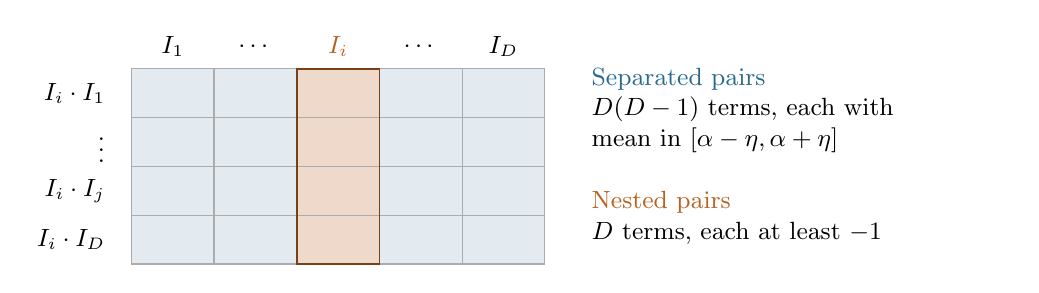
\begin{tikzpicture}[x=1.05cm,y=0.62cm,font=\small]
  \foreach \x in {0,1,2,3,4} {
    \foreach \y in {0,1,2,3} {
      \fill[parentblue!13] (\x,\y) rectangle +(1,1);
    }
  }
  \fill[childorange!24] (2,0) rectangle (3,4);
  \draw[gray!65,thin] (0,0) grid[xstep=1,ystep=1] (5,4);
  \draw[childorange!65!black,semithick] (2,0) rectangle (3,4);
  \node at (0.5,4.45) {$I_1$};
  \node at (1.5,4.45) {$\cdots$};
  \node[childorange] at (2.5,4.45) {$I_i$};
  \node at (3.5,4.45) {$\cdots$};
  \node at (4.5,4.45) {$I_D$};
  \node[anchor=east] at (-0.2,3.5) {$I_i\cdot I_1$};
  \node[anchor=east] at (-0.2,2.5) {$\vdots$};
  \node[anchor=east] at (-0.2,1.5) {$I_i\cdot I_j$};
  \node[anchor=east] at (-0.2,0.5) {$I_i\cdot I_D$};
  \node[anchor=west,align=left,text width=5.2cm] at (5.45,3.15)
    {\textcolor{parentblue}{Separated pairs}\\
     \(D(D-1)\) terms, each with\\
     mean in \([\alpha-\eta,\alpha+\eta]\)};
  \node[anchor=west,align=left,text width=5.2cm] at (5.45,0.95)
    {\textcolor{childorange}{Nested pairs}\\
     \(D\) terms, each at least \(-1\)};
\end{tikzpicture}
\caption{For fixed \(i\), the \((j,k)\) entry is
\(\ip{X_{I_i\cdot I_j}}{X_{I_k}}\). Rows index the children of
\(I_i\) and columns index all parents; the grid is schematic.
Only column \(i\) contains nested pairs, a fraction \(1/D\) of the
\(D^2\) terms.}
\label{fig:mixed-pairs}
\end{figure}

\step{6 (variance estimate)}
Expanding
\(\norm{z_i-m}^2=\norm{z_i}^2-2\ip{z_i}{m}+\norm m^2\) and inserting
\eqref{avg:parent-bound}--\eqref{avg:mixed-bound},
\begin{align}
  \EA\norm{z_i-m}^2
  &\le2\Bigl[\Bigl(1-\frac1D\Bigr)(\alpha+\eta)+\frac1D\Bigr]
     -2\Bigl[\Bigl(1-\frac1D\Bigr)(\alpha-\eta)-\frac1D\Bigr]\notag\\
  &=\frac4D+4\left(1-\frac1D\right)\eta
    \qquad(1\le i\le D).\label{avg:variance}
\end{align}
The terms in \(\alpha\) cancel, so no assumption on the sign or size of
\(\alpha\) is needed.

\step{7 (conclusion)}
Average \eqref{avg:displacement} over \(g\in A\) and apply
\eqref{avg:variance} to each \(i\):
\[
  \delta^2
  \le\frac{L^2}{D}\sum_{i=1}^D\EA\norm{z_i-m}^2
  \le L^2\left(\frac4D+4\left(1-\frac1D\right)\eta\right).
\]
Hence \(\delta^2/L^2-4/D\le4(1-1/D)\eta\). Dividing by
\(4(1-1/D)>0\) (recall \(D\ge2\)) gives \eqref{avg:boundary-bound}. Its
right-hand side is positive by \eqref{color:parameters} and does not
depend on \(A\).
\end{proof}

\begin{proof}[Proof of \cref{thm:main}]
Let \(c_0>0\) be the right-hand side of \eqref{avg:boundary-bound}. If
\(F\) were amenable, \eqref{eq:folner} with the fixed finite set \(S\) and
\(\varepsilon=c_0\) would give a nonempty finite \(A\subset F\) with
\(|hA\triangle A|/|A|<c_0\) for all \(h\in S\). This contradicts
\cref{avg:boundary}. Hence \(F\) is not amenable.
\end{proof}

\section{Consequences}\label{sec:consequences}

\Cref{thm:main} allows two companion results for nonamenable groups to be
applied. Neither is used in the proof of nonamenability.
Three symbols of the source are renamed here to avoid clashes:
the Hilbert space is \(\mathcal K\) (source: \(H\)), the similarity is
\(V\) (source: \(S\)), and the generating set is \(\Sigma\) (source: \(S\));
the connection operator is written \(\mathcal C_p\) (source: \(T_p\)).
In \cref{cor:percolation} only, \(p\) denotes a probability, not the
colouring of \cref{sec:coloring}.

\begin{corollary}\label{cor:nonunitarizable}
For every \(\varepsilon>0\), there are a separable complex Hilbert space
\(\mathcal K\) and a representation \(\pi:F\to\mathrm{GL}(\mathcal K)\)
such that \(\sup_{g\in F}\norm{\pi(g)}\le1+\varepsilon\), but no bounded
invertible operator \(V\) on \(\mathcal K\) makes every
\(V\pi(g)V^{-1}\) unitary.
\end{corollary}

\begin{proof}
The group \(F\) is countable, since each element is determined by finitely
many dyadic breakpoints and slopes in \(2^\Z\). It is nonamenable by
\cref{thm:main}. The conclusion follows from the companion
unitarizability theorem
\cite[Theorem~1.1]{OpenAIUnitarizability2026}.
\end{proof}

For a finite symmetric generating set \(\Sigma\subset F\setminus\{\id\}\),
let \(\mathcal G_\Sigma\) be the simple undirected Cayley graph with edges
\(\{x,xs\}\), \(s\in\Sigma\). In Bernoulli bond percolation on this graph,
each edge is independently open with probability \(p\). Write \(p_c\) for
the threshold for existence of an infinite open cluster and \(p_u\) for the
threshold for almost-sure uniqueness of the infinite open cluster. The
connection kernel \(\mathcal C_p(x,y)=\mathbb P_p(x\leftrightarrow y)\)
acts on counting-measure \(\ell^2(F)\), initially on finitely supported
functions by summation over \(y\); put
\(p_{2\to2}=\sup\{p\in[0,1]:\mathcal C_p\text{ is bounded on }\ell^2(F)\}\).

\begin{corollary}\label{cor:percolation}
For every such generating set \(\Sigma\),
\[
  \norm{\mathcal C_{p_c}}_{2\to2}<\infty,\qquad p_c<p_{2\to2}\le p_u.
\]
For each fixed \(p\in(p_c,p_u)\), there are almost surely infinitely many
infinite open clusters. Moreover, there are deterministic
\(p_c<p_1<p_2<1\), depending on \(\Sigma\), such that in the coupling with
independent uniform \([0,1]\) edge labels \(U_e\), opening \(e\) when
\(U_e\le p\), there are almost surely infinitely many infinite open
clusters simultaneously for every \(p\in[p_1,p_2]\).
\end{corollary}

\begin{proof}
Apply the companion percolation result
\cite[Corollary~1.2]{OpenAIPercolation2026} to \(F\), which is nonamenable
by \cref{thm:main}.
\end{proof}

\unverified{The proofs of \cref{cor:nonunitarizable,cor:percolation} consist
only of the two citations above. The source does not reproduce the cited
statements and I could not consult the companion papers, so I cannot confirm
that they say what is needed. What is needed is: for
\cref{cor:nonunitarizable}, that \emph{every} countable nonamenable group
has such a representation for each \(\varepsilon>0\); for
\cref{cor:percolation}, the displayed conclusions for \emph{every} Cayley
graph of a finitely generated nonamenable group. Both are strong general
statements, so these two corollaries should be read as conditional on the
companion papers.}

\appendix
\section{An explicit map with positive displacement}\label{app:auxiliary}

This appendix proves \cref{lem:displacement} directly, in the form of
\cref{aux:map} below (\(\delta=1/2\)). It is the Hilbert-space instance of
the Benyamini--Sternfeld theorem~\cite{BenyaminiSternfeld1983}. It is
logically independent of \cref{sec:dyadic,sec:coloring,sec:boundary}.
\emph{Notation.} Only \(H,B,f\) keep their meaning from the main text. All
other letters (\(a,b,q,c,d,r,t,\tau,\rho,G,\dots\)) are defined afresh here.
Compared with the source, the second curve parameter \(s\) is renamed
\(\tau\), the operator \(A\) is renamed \(W\), the constants \(K,M\) are
renamed \(K_\gamma,M_\gamma\), and \(Jv(t)\) is written \(v^\perp(t)\).

\begin{proposition}\label{aux:map}
Let \(H=L^2([0,1];\R^2)\), a real Hilbert space, and let
\(B=\{x\in H:\norm{x}\le1\}\). There is a globally Lipschitz map
\(f:B\to B\) such that
\[
  \norm{f(x)}=1,
  \qquad \norm{f(x)-x}\ge\frac12
  \quad(x\in B).
\]
\end{proposition}

\paragraph{Plan.}
We construct a Lipschitz map \(G:B\to H\) with \(\norm{G(x)}\ge\rho/4>0\)
everywhere and \(G(x)=x\) when \(\norm x\ge1/2\). Then
\(f(x)=-G(x)/\norm{G(x)}\) works. The identity map fails only because it
vanishes at \(0\). \(G\) modifies the identity inside a thin tube around a
curve \(\gamma\) through \(0\), sliding the zero away along the curve.
The curve's forward tail stays in a small ball yet never comes back close to
itself (\cref{aux:tube}). \Cref{aux:rotation} supplies rotations that keep
the modification from being cancelled by the component transverse to the
curve.

\subsection{The curve}

Define functions on \(\R\) by
\[
 a(t)=
 \begin{cases}
 t/8,&t\le2,\\
 5/16-(3-t)^2/16,&2<t<3,\\
 5/16,&t\ge3,
 \end{cases}
 \qquad
 \theta(t)=
 \begin{cases}
 0,&t\le1,\\
 (t-1)^2/2,&1<t<2,\\
 t-3/2,&t\ge2.
 \end{cases}
\]
For \(w\in[0,1]\) put
\[
 v(t)(w)=(\cos(\theta(t)w),\sin(\theta(t)w)),\quad
 v^\perp(t)(w)=(-\sin(\theta(t)w),\cos(\theta(t)w)),\quad
 \gamma(t)=a(t)v(t).
\]
Pointwise in \(w\), \(v(t)(w)\) and \(v^\perp(t)(w)\) are orthonormal in
\(\R^2\); hence \(\norm{v(t)}=1\) in \(H\) and \(\norm{\gamma(t)}=|a(t)|\).
Also \(\gamma(0)=0\).

\begin{center}
\begin{tabular}{lcccc}
\toprule
range & \(a\) & \(a'\) & \(\theta\) & \(\theta'\)\\
\midrule
\(t\le1\) & \(t/8\) & \(1/8\) & \(0\) & \(0\)\\
\(1\le t\le2\) & \(t/8\) & \(1/8\) & \((t-1)^2/2\) & \(t-1\)\\
\(2\le t\le3\) & \(5/16-(3-t)^2/16\) & \((3-t)/8\) & \(t-3/2\) & \(1\)\\
\(t\ge3\) & \(5/16\) & \(0\) & \(t-3/2\) & \(1\)\\
\bottomrule
\end{tabular}
\end{center}
The entries agree at \(t=1,2,3\) (for instance \(a(2)=1/4\) from both
sides, \(a'(2)=1/8\), \(a'(3)=0\), \(\theta(2)=1/2\), \(\theta'(1)=0\),
\(\theta'(2)=1\)). We read off:
\begin{enumerate}[label=(F\arabic*)]
\item \(a,\theta\) are \(C^1\); \(0\le a'\le1/8\) and \(0\le\theta'\le1\);
\(a'\) is \(\tfrac18\)-Lipschitz and \(\theta'\) is \(1\)-Lipschitz.
\item \(a\le5/16\) everywhere; \(a\) is strictly increasing on
\((-\infty,1]\); \(a(t)\ge1/8\) for \(t\ge1\); \(a(t)\ge1/4\) for
\(t\ge2\); \(a(t)=5/16\) for \(t\ge3\).
\item \(\theta=0\) on \((-\infty,1]\), \(\theta\) is strictly increasing on
\([1,\infty)\), and \(\theta(t)=t-3/2\) for \(t\ge2\).
\item The product \(a\theta'\) vanishes on \((-\infty,1]\), satisfies
\(0\le a\theta'\le5/16\), and is \(\tfrac7{16}\)-Lipschitz on \(\R\).
On \([1,\infty)\) we have \(0<a\le5/16\), \(0\le\theta'\le1\), so
\(|a\theta'(t)-a\theta'(\tau)|\le\tfrac5{16}|\theta'(t)-\theta'(\tau)|
+|a(t)-a(\tau)|\le(\tfrac5{16}+\tfrac18)|t-\tau|\). For
\(\tau\le1\le t\), compare with the value \(0\) at \(1\).
\end{enumerate}
By (F3), \(\gamma(t)=(t/8)\,v(0)\) for \(t\le1\), a straight line. By (F2),
\(\norm{\gamma(t)}\le5/16\) for \(t\ge1\).

The next lemma is used in the proof of \cref{aux:map}: it provides the tube
\(U\), the nearest-point parameter \(t(x)\), and the Lipschitz control
\eqref{aux:parameter}.

\begin{lemma}\label{aux:tube}
The curve \(\gamma\) is injective, has a bounded Lipschitz derivative, and
\[
 c:=\inf_{t\in\R}\norm{\gamma'(t)}=\frac18.
\]
Its unit tangent \(u(t)=\gamma'(t)/\norm{\gamma'(t)}\) is Lipschitz,
\(\ip{u(t)}{v(t)}\ge0\), and \(u(t)=v(t)\) for \(t\le1\).
There is a radius \(0<\rho<1/32\) such that every point in
\[
 U=\{x\in H:\dist(x,\gamma(\R))<\rho\}
\]
has a unique nearest point \(\gamma(t(x))\). Writing
\(e(x)=x-\gamma(t(x))\), we have \(e(x)\perp u(t(x))\), and
\begin{equation}\label{aux:parameter}
 |t(x)-t(y)|\le16\norm{x-y}
 \quad\text{if }x,y\in U\text{ and }\norm{x-y}<\rho.
\end{equation}
\end{lemma}

\begin{proof}
\step{1 (derivative in \(H\))}
For fixed \(w\in[0,1]\), the \(\R^2\)-valued function
\(t\mapsto\gamma(t)(w)\) is \(C^1\) by (F1), with derivative
\[
 g_w(t)=a'(t)\,v(t)(w)+a(t)\theta'(t)\,w\,v^\perp(t)(w).
\]
We claim \(|g_w(t)-g_w(\tau)|\le|t-\tau|\) for all \(w\in[0,1]\).
The unit vectors \(v(t)(w)\) and \(v^\perp(t)(w)\) have angle
\(\theta(t)w\), so each moves by at most
\(|\theta(t)-\theta(\tau)|w\le|t-\tau|\). By (F1), the first term changes
by at most \(|a'(t)-a'(\tau)|+\tfrac18|t-\tau|\le\tfrac14|t-\tau|\). By
(F4), the second changes by at most
\(\tfrac7{16}|t-\tau|+\tfrac5{16}|t-\tau|=\tfrac34|t-\tau|\).
Hence, by the fundamental theorem of calculus,
\(|\gamma(t)(w)-\gamma(\tau)(w)-(t-\tau)g_w(\tau)|\le\tfrac12|t-\tau|^2\)
uniformly in \(w\). Squaring and integrating over \(w\) gives the same
bound in the norm of \(H\). So \(\gamma\) is differentiable in \(H\) with
\[
 \gamma'(t)=a'(t)v(t)+a(t)\theta'(t)\,w\,v^\perp(t),
\]
and \(\norm{\gamma'(t)-\gamma'(\tau)}\le|t-\tau|\). Write
\(K_\gamma=\Lip(\gamma')\le1\).

\step{2 (speed)}
Since \(v\perp v^\perp\) pointwise and \(\int_0^1w^2\,dw=\tfrac13\),
\[
 \norm{\gamma'(t)}^2=a'(t)^2+\frac{a(t)^2\theta'(t)^2}{3}.
\]
For \(t\le2\) the first term is \(1/64\). For \(t\ge2\) the second term is
at least \((1/4)^2/3=1/48>1/64\) by (F2), (F3). For \(t\le1\) the second
term vanishes. So \(c=1/8\), attained for \(t\le1\). Also
\(M_\gamma:=\sup_t\norm{\gamma'(t)}\le(1/64+25/768)^{1/2}<\infty\).

\step{3 (\(u\) and \(v\))}
For \(\norm y,\norm{y'}\ge\mu>0\) one has
\begin{equation}\label{aux:normalize}
 \Bigl\|\frac{y}{\norm y}-\frac{y'}{\norm{y'}}\Bigr\|
 \le\frac{\norm{y-y'}}{\norm y}
    +\frac{\bigl|\norm{y'}-\norm y\bigr|}{\norm y}
 \le\frac2\mu\norm{y-y'}.
\end{equation}
With \(\mu=c\), \(u\) is Lipschitz; write \(K_u=\Lip(u)\). By Step~1's
angle bound, \(v\) is \(1\)-Lipschitz. Since \(\ip{v^\perp(t)(w)}{v(t)(w)}=0\)
pointwise, \(\ip{\gamma'(t)}{v(t)}=a'(t)\), so
\(\ip{u(t)}{v(t)}=a'(t)/\norm{\gamma'(t)}\ge0\). For \(t\le1\),
\(\gamma'(t)=\tfrac18v(t)\), so \(u(t)=v(t)\).

\step{4 (injectivity)}
Let \(\sinc(\omega)=\sin(\omega)/\omega\) for \(\omega\ne0\) and
\(\sinc(0)=1\). Integrating \(\cos((\theta(t)-\theta(\tau))w)\) over
\(w\in[0,1]\) gives
\begin{equation}\label{aux:sinc}
 \ip{v(\tau)}{v(t)}=\sinc(\theta(t)-\theta(\tau)),\qquad
 \norm{\gamma(t)-\gamma(\tau)}^2
   =a(t)^2+a(\tau)^2-2a(t)a(\tau)\sinc(\theta(t)-\theta(\tau)).
\end{equation}
Let \(\tau<t\). If \(t\le1\), then
\(\norm{\gamma(t)-\gamma(\tau)}=(t-\tau)/8\ne0\). If \(t>1\), then
\(\theta(t)>\theta(\tau)\) by (F3). Since \(|\sinc(\omega)|<1\) for
\(\omega\ne0\), the unit vectors \(v(\tau),v(t)\) are linearly independent
(equality case of Cauchy--Schwarz). So \(a(\tau)v(\tau)=a(t)v(t)\) would
force \(a(t)=0\), contradicting \(a(t)\ge1/8\).

\step{5 (uniform separation)}
We claim
\begin{equation}\label{aux:separation}
 \sigma(d):=\inf_{|t-\tau|\ge d}\norm{\gamma(t)-\gamma(\tau)}>0
 \qquad(d>0).
\end{equation}
Otherwise there are \(\tau_n<t_n\) with \(t_n-\tau_n\ge d\) and
\(\norm{\gamma(t_n)-\gamma(\tau_n)}\to0\). Pass to a subsequence with
\(\tau_n\to\tau_*\), \(t_n\to t_*\) in \([-\infty,+\infty]\);
\(\tau_*\le t_*\).
\begin{itemize}
\item \emph{Both finite.} Then \(t_*-\tau_*\ge d\) and, by continuity,
\(\gamma(t_*)=\gamma(\tau_*)\), contradicting Step~4.
\item \emph{\(t_*=-\infty\)} (so \(\tau_*=-\infty\)). Eventually both
parameters are \(\le1\) and the distance is \((t_n-\tau_n)/8\ge d/8\).
\item \emph{\(\tau_*=-\infty<t_*\).} Then
\(\norm{\gamma(\tau_n)}=|\tau_n|/8\to\infty\) while
\(\norm{\gamma(t_n)}=|a(t_n)|\) stays bounded.
\item \emph{\(\tau_*\) finite, \(t_*=+\infty\).} Then
\(\theta(t_n)-\theta(\tau_n)\to\infty\), so the \(\sinc\) term in
\eqref{aux:sinc} tends to \(0\). Since \(a(t_n)=5/16\) eventually, the
squared distances tend to \(a(\tau_*)^2+(5/16)^2>0\).
\item \emph{Both \(+\infty\).} Eventually both are \(\ge3\), so by (F2),
(F3) and \eqref{aux:sinc}
\[
 \norm{\gamma(t_n)-\gamma(\tau_n)}^2
 =2(5/16)^2\bigl(1-\sinc(t_n-\tau_n)\bigr)
 \ge2(5/16)^2\bigl(1-\sup_{\omega\ge d}\sinc(\omega)\bigr)>0.
\]
The supremum is less than \(1\): \(\sinc\) is continuous, \(\sinc(\omega)<1\)
for \(\omega>0\), and \(|\sinc(\omega)|\le1/\omega\).
\end{itemize}
Every case contradicts the choice of the sequences.

\step{6 (tangent estimate; choice of \(d\) and \(\rho\))}
For a unit vector \(\xi\in H\), the scalar function
\(s\mapsto\ip{\gamma(s)}{\xi}\) is \(C^1\) with derivative
\(\ip{\gamma'(s)}{\xi}\), so
\(\ip{\gamma(t)-\gamma(\tau)-(t-\tau)\gamma'(\tau)}{\xi}
=\int_\tau^t\ip{\gamma'(s)-\gamma'(\tau)}{\xi}\,ds\). Taking the supremum
over \(\xi\),
\[
 \norm{\gamma(t)-\gamma(\tau)-(t-\tau)\gamma'(\tau)}
 \le\frac{K_\gamma}2|t-\tau|^2 .
\]
Choose \(d>0\) with \(K_\gamma d\le c/2\). Pairing with \(u(\tau)\), and
using \(\ip{\gamma'(\tau)}{u(\tau)}=\norm{\gamma'(\tau)}\ge c\), we get for
\(|t-\tau|\le d\)
\begin{equation}\label{aux:tangent}
 |\ip{\gamma(t)-\gamma(\tau)}{u(\tau)}|
 \ge c|t-\tau|-\frac{K_\gamma d}{2}|t-\tau|
 \ge\frac{3c}{4}|t-\tau|.
\end{equation}
Now choose \(\rho>0\) with
\begin{equation}\label{aux:radius}
 \rho<\frac1{32},\qquad 4\rho<\sigma(d),\qquad \rho K_u<\frac c4.
\end{equation}

\step{7 (nearest points exist and the residual is orthogonal)}
Let \(x\in U\) and let \(\gamma(t_n)\) be a minimizing sequence for
\(\dist(x,\gamma(\R))<\rho\). Late terms satisfy
\(\norm{x-\gamma(t_n)}<2\rho\), so they are pairwise less than
\(4\rho<\sigma(d)\) apart. By \eqref{aux:separation} their parameters
differ by less than \(d\). So the late \(t_n\) lie in a compact interval,
and a convergent subsequence gives a parameter attaining the minimum.
At any minimizing parameter \(t\),
\(0=\frac{d}{dt}\norm{x-\gamma(t)}^2=-2\ip{x-\gamma(t)}{\gamma'(t)}\),
so \(x-\gamma(t)\perp u(t)\).

\step{8 (Lipschitz parameter and uniqueness)}
Let \(x,y\in U\) with \(\norm{x-y}<\rho\). Take any minimizing parameters
\(t\) for \(x\) and \(\tau\) for \(y\), and write \(x=\gamma(t)+e_t\),
\(y=\gamma(\tau)+e_\tau\), with \(\norm{e_t},\norm{e_\tau}<\rho\). Then
\(\norm{\gamma(t)-\gamma(\tau)}<3\rho<\sigma(d)\), so \(|t-\tau|<d\).
By Step~7, \(\ip{e_\tau}{u(\tau)}=0\) and
\(\ip{e_t}{u(\tau)}=\ip{e_t}{u(\tau)-u(t)}\). Hence, by
\eqref{aux:tangent} and \eqref{aux:radius},
\begin{align*}
 \norm{x-y}\ge|\ip{x-y}{u(\tau)}|
 &\ge |\ip{\gamma(t)-\gamma(\tau)}{u(\tau)}|
       -|\ip{e_t}{u(\tau)-u(t)}|\\
 &\ge\left(\frac{3c}{4}-\rho K_u\right)|t-\tau|
 \ge\frac c2|t-\tau|=\frac{|t-\tau|}{16}.
\end{align*}
Taking \(y=x\) shows that the minimizing parameter is unique; call it
\(t(x)\). The same inequality is \eqref{aux:parameter}.
\end{proof}

\subsection{Rotations}

The next lemma is used in the lower bound \eqref{aux:nonzero}. A residual
\(e\perp u(t)\) is carried to \(R_te\perp v(t)\), so that changing the
coefficient along \(v(t)\) cannot be cancelled by the residual.

\begin{lemma}\label{aux:rotation}
There is a family of orthogonal operators \(R_t:H\to H\), Lipschitz
in operator norm, such that \(R_tu(t)=v(t)\) and \(R_t\) is the identity
for \(t\le1\).
\end{lemma}

\begin{proof}
Suppress \(t\) and put \(\kappa=\ip{u}{v}\ge0\) (\cref{aux:tube}). Define
\[
 W\xi=v\ip{u}{\xi}-u\ip{v}{\xi}\quad(\xi\in H),
 \qquad R=\mathrm{Id}+W+\frac{W^2}{1+\kappa}.
\]
\step{1}
\(W\) is skew-adjoint:
\(\ip{W\xi}{\zeta}=\ip v\zeta\ip u\xi-\ip u\zeta\ip v\xi
=-\ip{\xi}{W\zeta}\).

\step{2 (\(u,v\) independent)}
\(Wu=v-\kappa u\) and \(Wv=\kappa v-u\), so
\(W^2u=(\kappa v-u)-\kappa(v-\kappa u)=-(1-\kappa^2)u\) and
\(W^2v=\kappa(\kappa v-u)-(v-\kappa u)=-(1-\kappa^2)v\). Thus on
\(\operatorname{span}\{u,v\}\), \(W^2=-(1-\kappa^2)\mathrm{Id}\) and
\(R=\mathrm{Id}+W-(1-\kappa)\mathrm{Id}=\kappa\,\mathrm{Id}+W\).
This restriction is orthogonal, since by Step~1
\((\kappa\,\mathrm{Id}+W)^*(\kappa\,\mathrm{Id}+W)
=\kappa^2\mathrm{Id}-W^2=\mathrm{Id}\). Also
\(Ru=\kappa u+v-\kappa u=v\). On the orthogonal complement of the span,
\(W=0\) and \(R=\mathrm{Id}\). So \(R\) is orthogonal on \(H\).

\step{3 (\(u,v\) dependent)}
Unit vectors with \(\kappa\ge0\) that are dependent are equal. Then
\(W=0\), \(R=\mathrm{Id}\), and \(Ru=v\). By \cref{aux:tube} this is the
case for \(t\le1\).

\step{4 (Lipschitz)}
\(u,v\) are Lipschitz unit vectors, so \(t\mapsto W_t\) and
\(t\mapsto\kappa(t)\) are Lipschitz and \(\norm{W_t}\le2\). Since
\(1+\kappa\ge1\), \(t\mapsto1/(1+\kappa(t))\) is Lipschitz and bounded.
The formula for \(R\) then gives the claim, including where \(u=v\).
\end{proof}

\subsection{Proof of \cref{aux:map}}

Fix \(\rho\), \(U\), \(t(\cdot)\), \(e(\cdot)\) from \cref{aux:tube} and
\(R_t\) from \cref{aux:rotation}. Set
\[
 b(t)=\min\{a(t),-1/8\},\qquad
 q(t)=b(t)-a(t)=-\max\{a(t)+1/8,0\}.
\]
By (F2), \(|q(t)|\le5/16+1/8=7/16\). Also \(\Lip(q)\le\Lip(a)\le1/8\).
Let \(\beta,\chi:[0,\infty)\to[0,1]\) be the continuous piecewise linear
functions
\[
 \beta(r)=
 \begin{cases}
 1,&r\le\rho/4,\\
 2-4r/\rho,&\rho/4<r<\rho/2,\\
 0,&r\ge\rho/2,
 \end{cases}
 \qquad
 \chi(r)=
 \begin{cases}
 1,&r\le\rho/2,\\
 2-2r/\rho,&\rho/2<r<\rho,\\
 0,&r\ge\rho.
 \end{cases}
\]
Define \(G:B\to H\) by \(G(x)=x\) for \(x\notin U\). For \(x\in B\cap U\),
write \(t=t(x)\), \(e=e(x)\), \(r=\norm e=\dist(x,\gamma(\R))\), and set
\begin{equation}\label{aux:G}
 \begin{split}
 G(x)&=\gamma(t)+\beta(r)q(t)v(t)
       +\bigl((1-\chi(r))\mathrm{Id}+\chi(r)R_t\bigr)e\\
 &=x+\beta(r)q(t)v(t)+\chi(r)(R_t-\mathrm{Id})e .
 \end{split}
\end{equation}
The two lines agree because \(x=\gamma(t)+e\).

\begin{proof}[Proof of \cref{aux:map}]
\step{1 (\(G\) is globally Lipschitz on \(B\))}
We treat pairs \(x,y\in B\) by cases.

\emph{(a) \(x,y\in U\), \(\norm{x-y}<\rho\).} By \eqref{aux:parameter},
\(|t(x)-t(y)|\le16\norm{x-y}\). Hence
\(\norm{e(x)-e(y)}\le\norm{x-y}+\norm{\gamma(t(x))-\gamma(t(y))}
\le(1+16M_\gamma)\norm{x-y}\), with \(M_\gamma\) from Step~2 of
\cref{aux:tube}. The distance \(r(x)=\dist(x,\gamma(\R))\) is
\(1\)-Lipschitz. So each factor in the second line of \eqref{aux:G} is
Lipschitz on such pairs, with constants independent of the pair, and is
uniformly bounded: \(\beta(r),\chi(r)\in[0,1]\); \(|q|\le7/16\);
\(\norm v=1\); \(\norm{R_t-\mathrm{Id}}\le2\); \(\norm e<\rho\). A product
of bounded Lipschitz factors is Lipschitz, so there is one constant for all
such pairs.

\emph{(b) \(\norm{x-y}\ge\rho\).} For all \(x\in B\),
\(\norm{G(x)}\le1+7/16+2\rho<3/2\) (using \(\rho<1/32\)). So
\(\norm{G(x)-G(y)}\le3\le(3/\rho)\norm{x-y}\).

\emph{(c) \(x\in U\), \(y\notin U\), \(\norm{x-y}<\rho\).}
Both cutoffs satisfy \(\beta(r)\le\chi(r)\le2(\rho-r)/\rho\) for
\(r<\rho\): for \(r\le\rho/2\) the right side is \(\ge1\), and for
\(r>\rho/2\) it equals \(\chi(r)\) while \(\beta(r)=0\). Hence, from
\eqref{aux:G},
\[
 \norm{G(x)-x}\le\frac{2(\rho-r)}{\rho}\Bigl(\frac7{16}+2\rho\Bigr)
 =\left(\frac{7}{8\rho}+4\right)(\rho-r).
\]
Since \(\dist(\cdot,\gamma(\R))\) is \(1\)-Lipschitz and
\(\dist(y,\gamma(\R))\ge\rho\), we get \(\rho-r\le\norm{x-y}\). With
\(G(y)=y\), this gives
\(\norm{G(x)-G(y)}\le(\tfrac7{8\rho}+5)\norm{x-y}\).

\emph{(d) \(x,y\notin U\).} \(G\) is the identity.

\step{2 (lower bound)}
We claim
\begin{equation}\label{aux:nonzero}
 \norm{G(x)}\ge\rho/4\qquad(x\in B).
\end{equation}
\emph{Outside \(U\):} since \(0=\gamma(0)\),
\(\norm{G(x)}=\norm x\ge\dist(x,\gamma(\R))\ge\rho\).

\emph{Inside \(U\), \(r\le\rho/2\):} here \(\chi(r)=1\), so
\(G(x)=(a(t)+\beta(r)q(t))v(t)+R_te\). Since \(e\perp u(t)\), \(R_t\) is
orthogonal and \(R_tu(t)=v(t)\), we have
\(\ip{R_te}{v(t)}=\ip{e}{u(t)}=0\) and \(\norm{R_te}=r\). Thus
\(\norm{G(x)}^2=(a+\beta q)^2+r^2\). If \(r\le\rho/4\), then \(\beta=1\)
and \(a+q=b\le-1/8\), so \(\norm{G(x)}\ge1/8>\rho/4\). If
\(\rho/4\le r\le\rho/2\), then \(\norm{G(x)}\ge r\ge\rho/4\).

\emph{Inside \(U\), \(\rho/2\le r<\rho\):} here \(\beta(r)=0\), and the
last term in the first line of \eqref{aux:G} has norm at most \(r<\rho\).
If \(t>1\), then \(\norm{\gamma(t)}=a(t)\ge1/8\) by (F2), so
\(\norm{G(x)}\ge1/8-\rho>\rho/4\). If \(t\le1\), then
\(R_t=\mathrm{Id}\) and \(u(t)=v(t)\), so \(G(x)=a(t)v(t)+e\) with
\(e\perp v(t)\), and \(\norm{G(x)}\ge r\ge\rho/2\).

\step{3 (\(G(x)=x\) whenever \(\norm x\ge1/2\))}
Outside \(U\) this is the definition. Inside \(U\),
\[
 |a(t)|=\norm{\gamma(t)}\ge\norm x-r>1/2-\rho>5/16.
\]
Since \(a\le5/16\) everywhere, this forces \(a(t)<-5/16<-1/8\), hence
\(t\le1\). Thus \(q(t)=0\) and \(R_t=\mathrm{Id}\), and the second line of
\eqref{aux:G} gives \(G(x)=x\).

\step{4 (the map \(f\))}
Define \(f(x)=-G(x)/\norm{G(x)}\). By \eqref{aux:nonzero} and
\eqref{aux:normalize} with \(\mu=\rho/4\), normalization is
\((8/\rho)\)-Lipschitz on the range of \(G\), so \(f\) is globally
Lipschitz by Step~1, and \(\norm{f(x)}=1\). If \(\norm x<1/2\), then
\(\norm{f(x)-x}\ge1-\norm x>1/2\). Otherwise \(G(x)=x\) by Step~3, so
\(f(x)=-x/\norm x\) and \(\norm{f(x)-x}=1+\norm x\ge3/2\).
\end{proof}

\Cref{aux:map} gives \cref{lem:displacement} with \(H=L^2([0,1];\R^2)\) and
\(\delta=1/2\).

\section*{Verification checklist}

The steps that carry the proof, in the order a sceptical reader should
check them:

\begin{enumerate}
\item \textbf{Order of choices.} \(S\) is fixed before \(A\); only the
level \(n\) depends on \(A\); the final constant involves only
\(\delta,L,D\). See the paragraph ``The finite set \(S\)'' and the opening
of the proof of \cref{avg:boundary}.
\item \textbf{Exact transport \(X_I(g)=X_{I_1}(h_{I,J}g)\).} It rests on
\cref{dyad:cov} (note \(hg=h\circ g\) and left translation in
\eqref{eq:folner}) and on admissibility at both \(g\) and \(hg\). See
Step~1 of \cref{avg:boundary}.
\item \textbf{Which pairs are separated.} Cross-scale pairs (descendant of
\(I_i\) with parent \(I_k\), \(k\ne i\)) are separated, and only \(D\) of
the \(D^2\) mixed pairs are nested. See \cref{color:pairs} and
\eqref{avg:mixed-bound}.
\item \textbf{Recursion identity \(X_{I_i}=f(z_i)\).} It needs
\((T_{I_i})_{I_j}=T_{I_i\cdot I_j}\) (\cref{dyad:restr}(c)) and
well-foundedness of \(p\) (\cref{color:wd}). See Step~3 of
\cref{avg:boundary}.
\item \textbf{The algebra.} \eqref{avg:parent-bound}--\eqref{avg:mixed-bound}
imply \eqref{avg:variance} with \(\alpha\) cancelling; then
\eqref{avg:displacement} and the rearrangement in Step~7.
\item \textbf{Existence of the transports.} \Cref{dyad:transport} needs
internal intervals and positive gaps so that all three gaps are
nondegenerate.
\item \textbf{The displacement map (only if \cref{lem:displacement} is not
taken from \cite{BenyaminiSternfeld1983}).} Check the uniform separation
\eqref{aux:separation}, especially the case where both parameters tend to
\(+\infty\), then the lower bound \eqref{aux:nonzero}, and Step~3 of the
proof of \cref{aux:map}.
\item \textbf{Scope.} \Cref{cor:nonunitarizable,cor:percolation} depend on
companion papers not checked here; see the boxed note in
\cref{sec:consequences}.
\end{enumerate}

\bibliographystyle{plain}
\bibliography{sources}
\end{document}
